\documentclass[aspectratio=169,10pt]{beamer}
\usepackage[utf8]{inputenc}
\usepackage[ngerman]{babel}
\usepackage{csquotes}
\usepackage{graphicx}
\usepackage{booktabs}
\usepackage{hyperref}
\usepackage{siunitx}

\usetheme{HM} % our custom theme

% Define custom colors:

% 1) Change the primary colour (hex HTML model):
% \sethmprimarycolor[HTML]{0077CC}

% 2) Set example block title/body colours (title, body):
% \sethmexampleblockcolors[HTML]{00AA66}{F0FFF0}

% 3) Set alert block title/body colours (title, body):
% \sethmalertblockcolors[HTML]{FF7700}{FFF4E6}

% Frametitlet spacing (defaults in theme; override below if needed):
% \sethmframetitletop{4mm} % top spacing (uncomment to change)
% \sethmframetitleleft{6mm} % left spacing (defaults to same as top)

% --- Meta ---
\title{Titel der Präsentation}
\subtitle{Optionaler Untertitel oder Slogan}
\author{Vorname Nachname}
\institute{Organisation oder Unternehmen \\ Abteilung oder Fakultät}
\date{\today}

% Footer text (appears centered in the footline)
\sethmfooter{© Autorenteam – Fakultät BW}

% If your logo has a different filename, set it here:
% \sethmlogo{hm_logo.pdf}

% Optional: separate footer logo (falls back to \sethmlogo if not set)
% To use: uncomment and set your file name
% \sethmfooterlogo{hm_footer_logo.png}

% Optional: table of contents style: numbers | bullets | none (default: numbers)
% \sethmtocstyle{bullets}

\begin{document}

\begin{frame}[plain]
  \titlepage
\end{frame}

\begin{frame}{Inhalt}
  \tableofcontents
\end{frame}

\section{Einführung}
\begin{frame}{Einführung}
\begin{itemize}
  \item Stellen Sie hier die wichtigsten Punkte Ihrer Präsentation vor.
  \item Verwenden Sie kurze, prägnante Aussagen und ergänzen Sie sie ggf. um Stichworte.
  \item Betonen Sie zentrale Kennzahlen oder Ergebnisse mit \textbf{fetter Schrift}.
\end{itemize}
\end{frame}

\section{Beispielblöcke}
\begin{frame}{Beispielblöcke}
\begin{block}{Hinweis}
  Neutrale graue Kästen für strukturierte Inhalte.
\end{block}
\begin{exampleblock}{Beispiel}
  Praxisbeispiel – kurze, klare Aussage.
\end{exampleblock}
\end{frame}

\section{Zweispaltiges Layout}
\begin{frame}{Zweispaltiges Layout}
\begin{columns}[T] % [T] für Top-Alignment
  \begin{column}{0.48\textwidth}
    \textbf{Linke Spalte}
    \begin{itemize}
      \item Für Vergleiche geeignet
      \item Text und Aufzählungen
      \item Strukturierte Argumente
    \end{itemize}
  \end{column}
  \hfill
  \begin{column}{0.48\textwidth}
    \textbf{Rechte Spalte}
    \begin{itemize}
      \item Gegenüberstellung
      \item Alternative Ansätze
      \item Pro und Contra
    \end{itemize}
  \end{column}
\end{columns}
\end{frame}

\section{Bilder}
\begin{frame}{Einzelnes Bild mit Beschreibung}
\begin{figure}
  \centering
  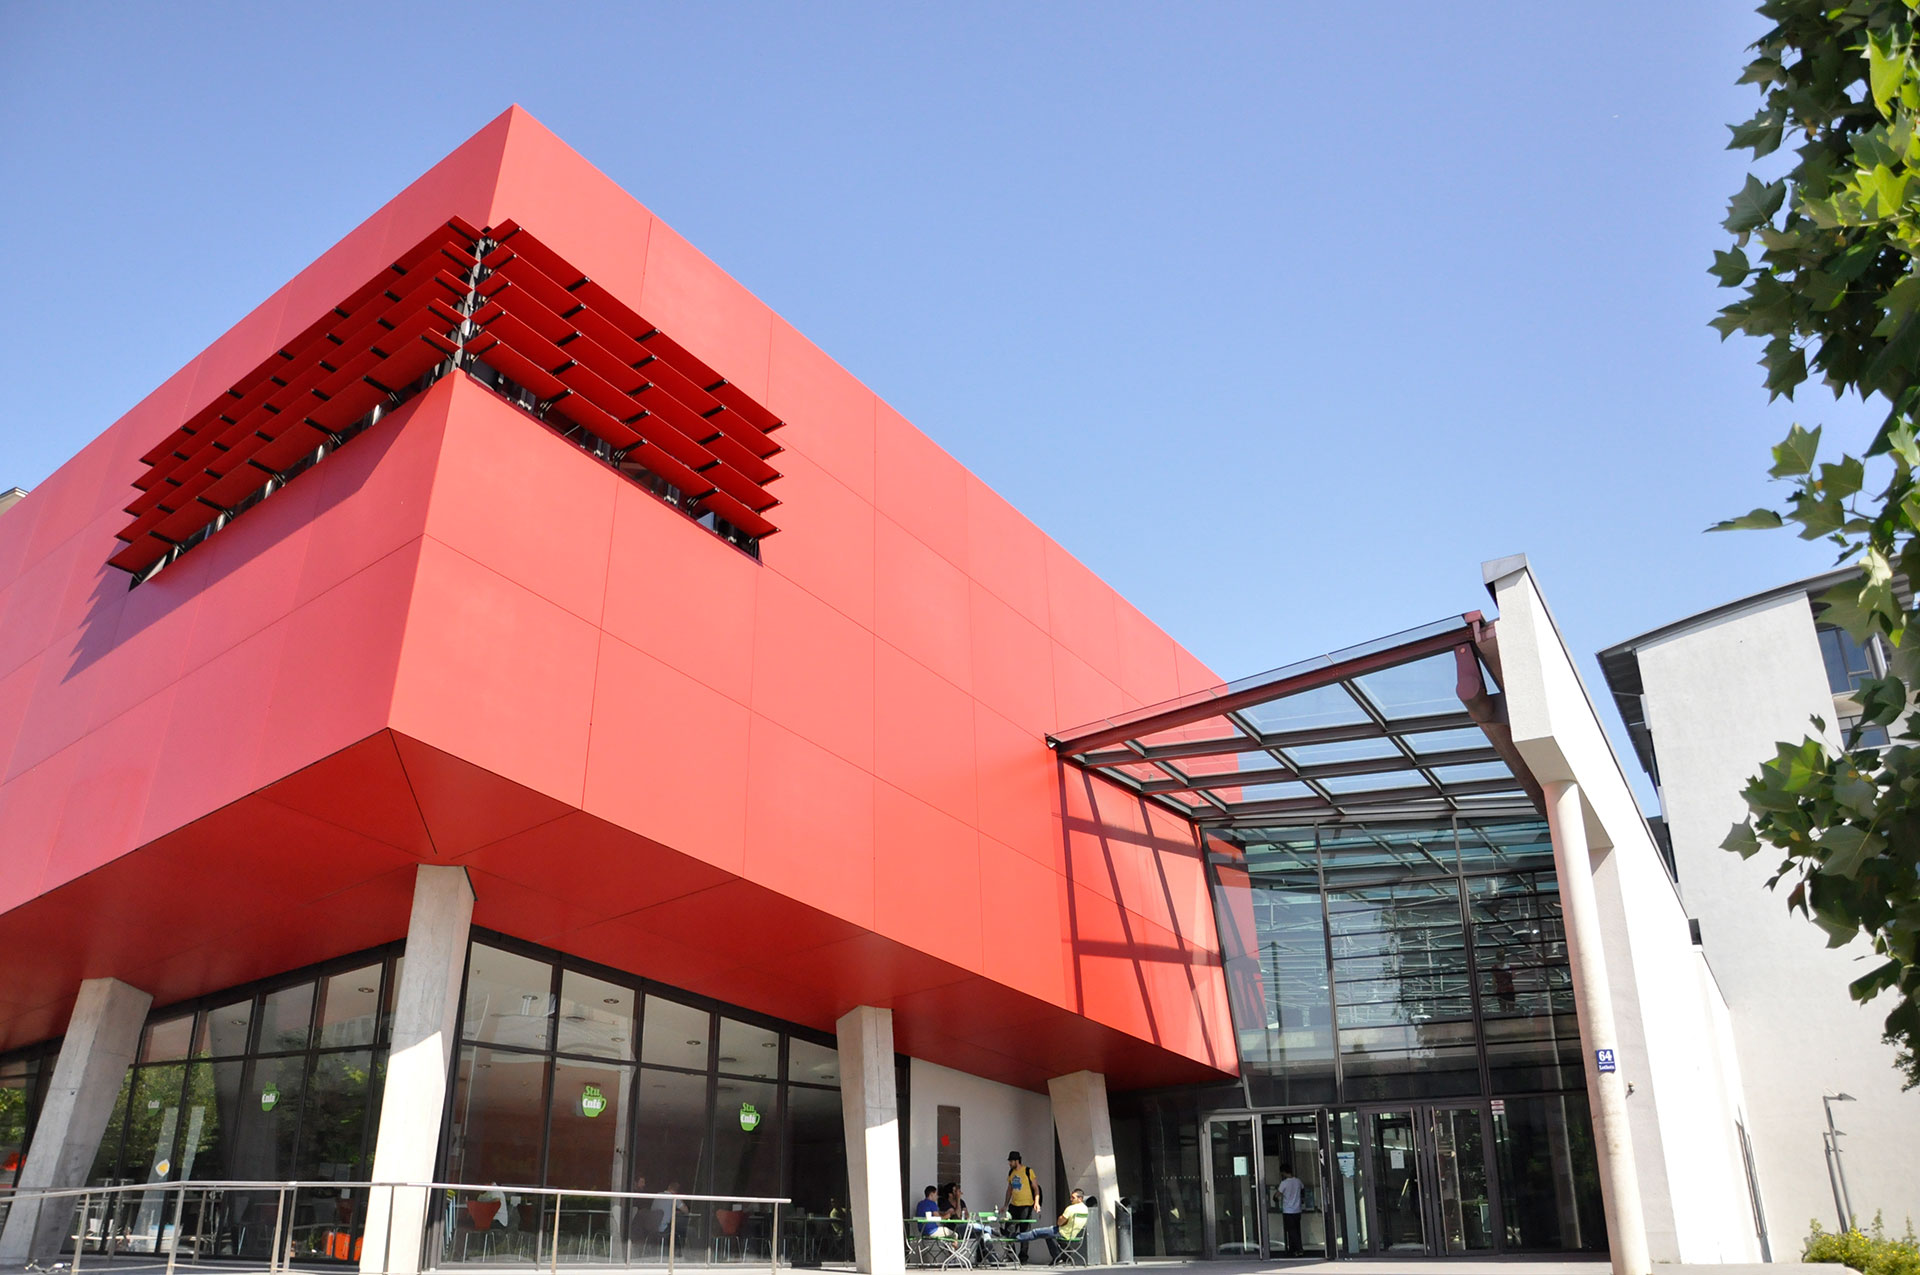
\includegraphics[width=0.6\textwidth]{assets/dm_roter_wuerfel_ben_steinig.jpg}
  \caption{Ein roter Würfel – ideal für Symbolik und visuelle Metaphern}
\end{figure}
\end{frame}

\begin{frame}{Bild und Text nebeneinander}
\begin{columns}[c]
  \begin{column}{0.5\textwidth}
    \begin{itemize}
      \item Kombinieren Sie Bild und Text
      \item Ideal für Erklärungen
      \item Visuelle Unterstützung
      \item Platzsparend und übersichtlich
    \end{itemize}
  \end{column}
  \begin{column}{0.45\textwidth}
    \begin{figure}
      \centering
      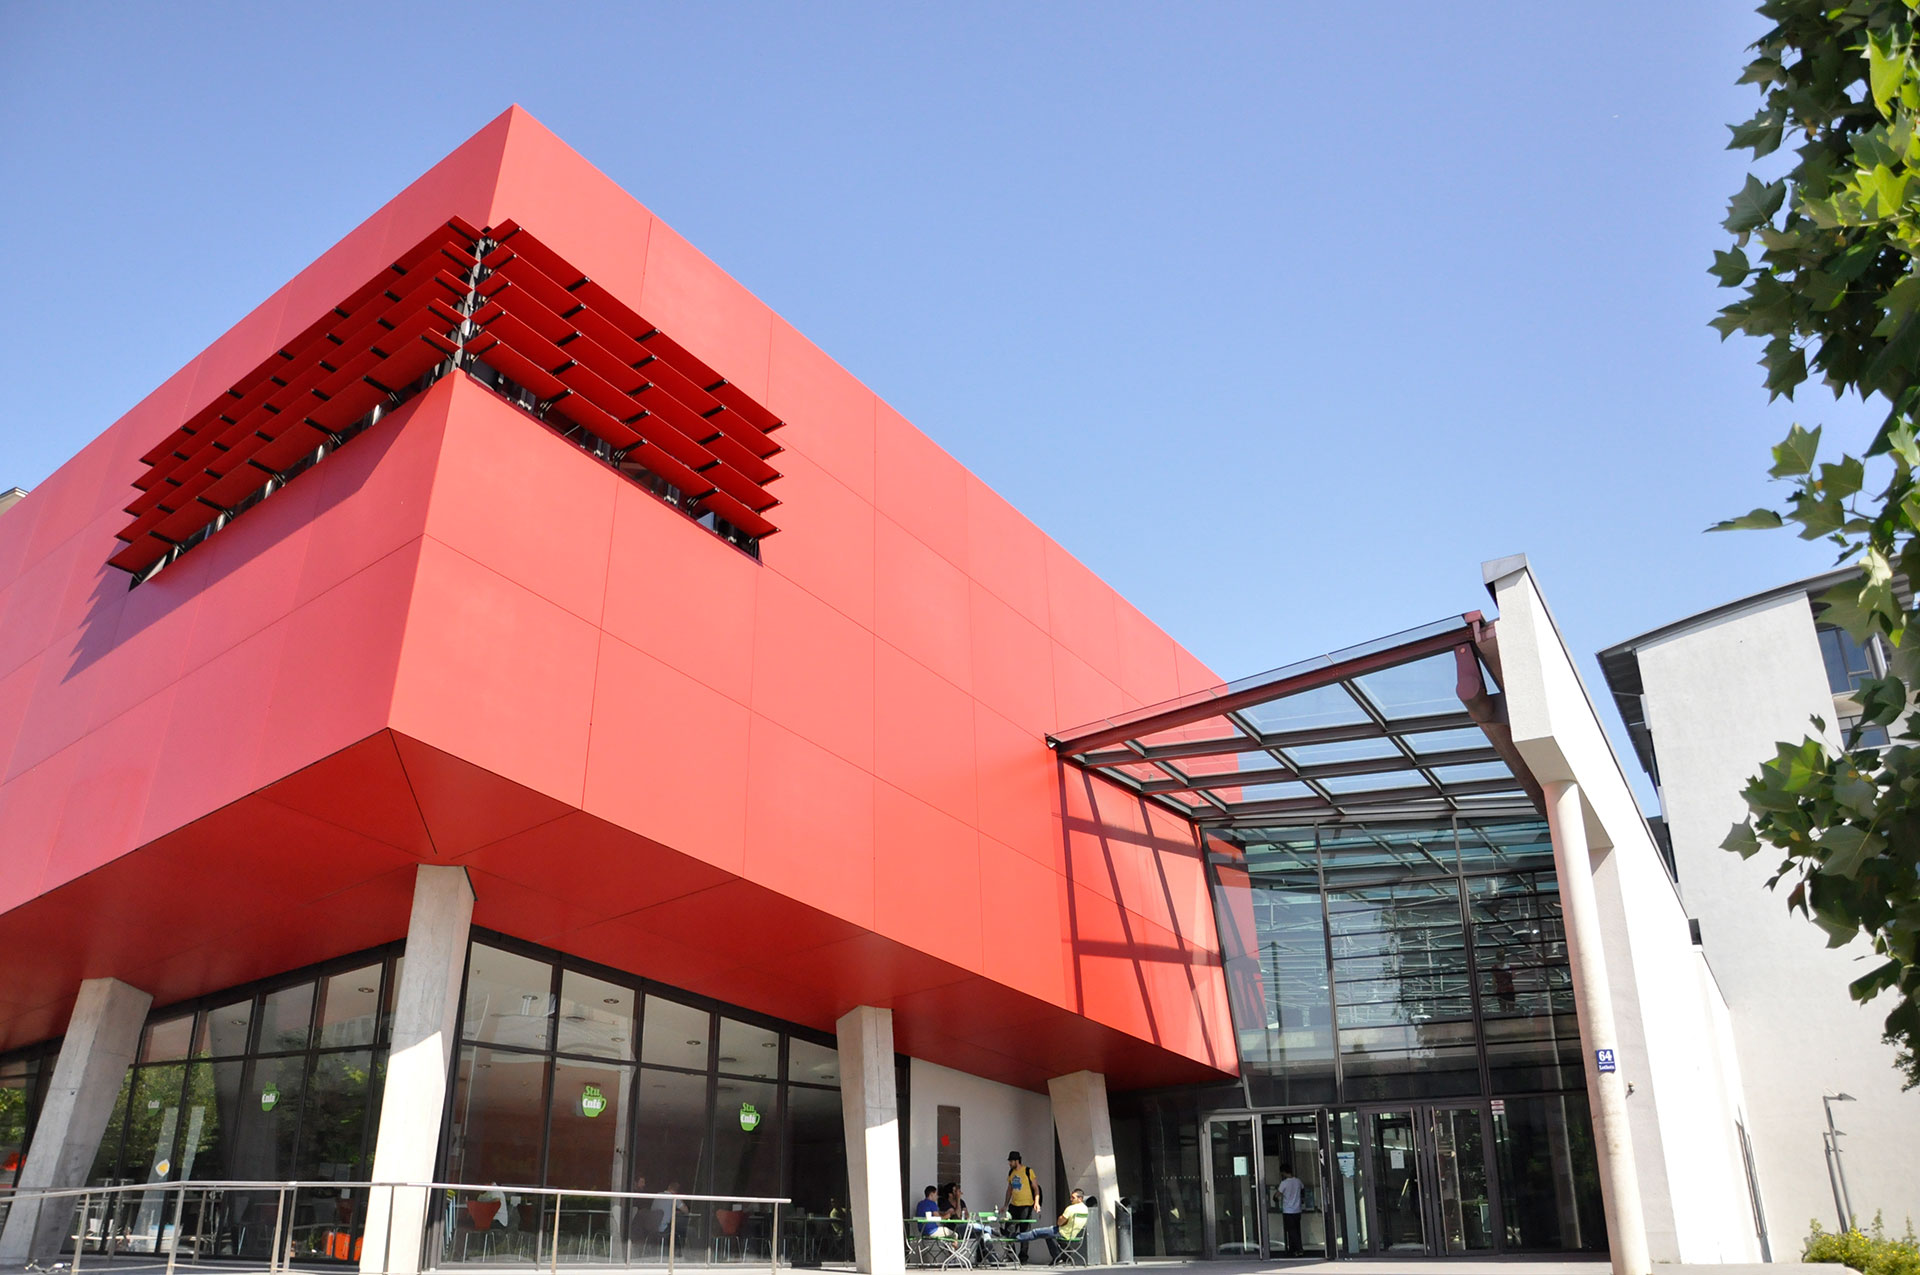
\includegraphics[width=\textwidth]{assets/dm_roter_wuerfel_ben_steinig.jpg}
      \caption{Roter Würfel}
    \end{figure}
  \end{column}
\end{columns}
\end{frame}

\begin{frame}{Zwei Bilder nebeneinander}
\begin{columns}[c]
  \begin{column}{0.48\textwidth}
    \begin{figure}
      \centering
      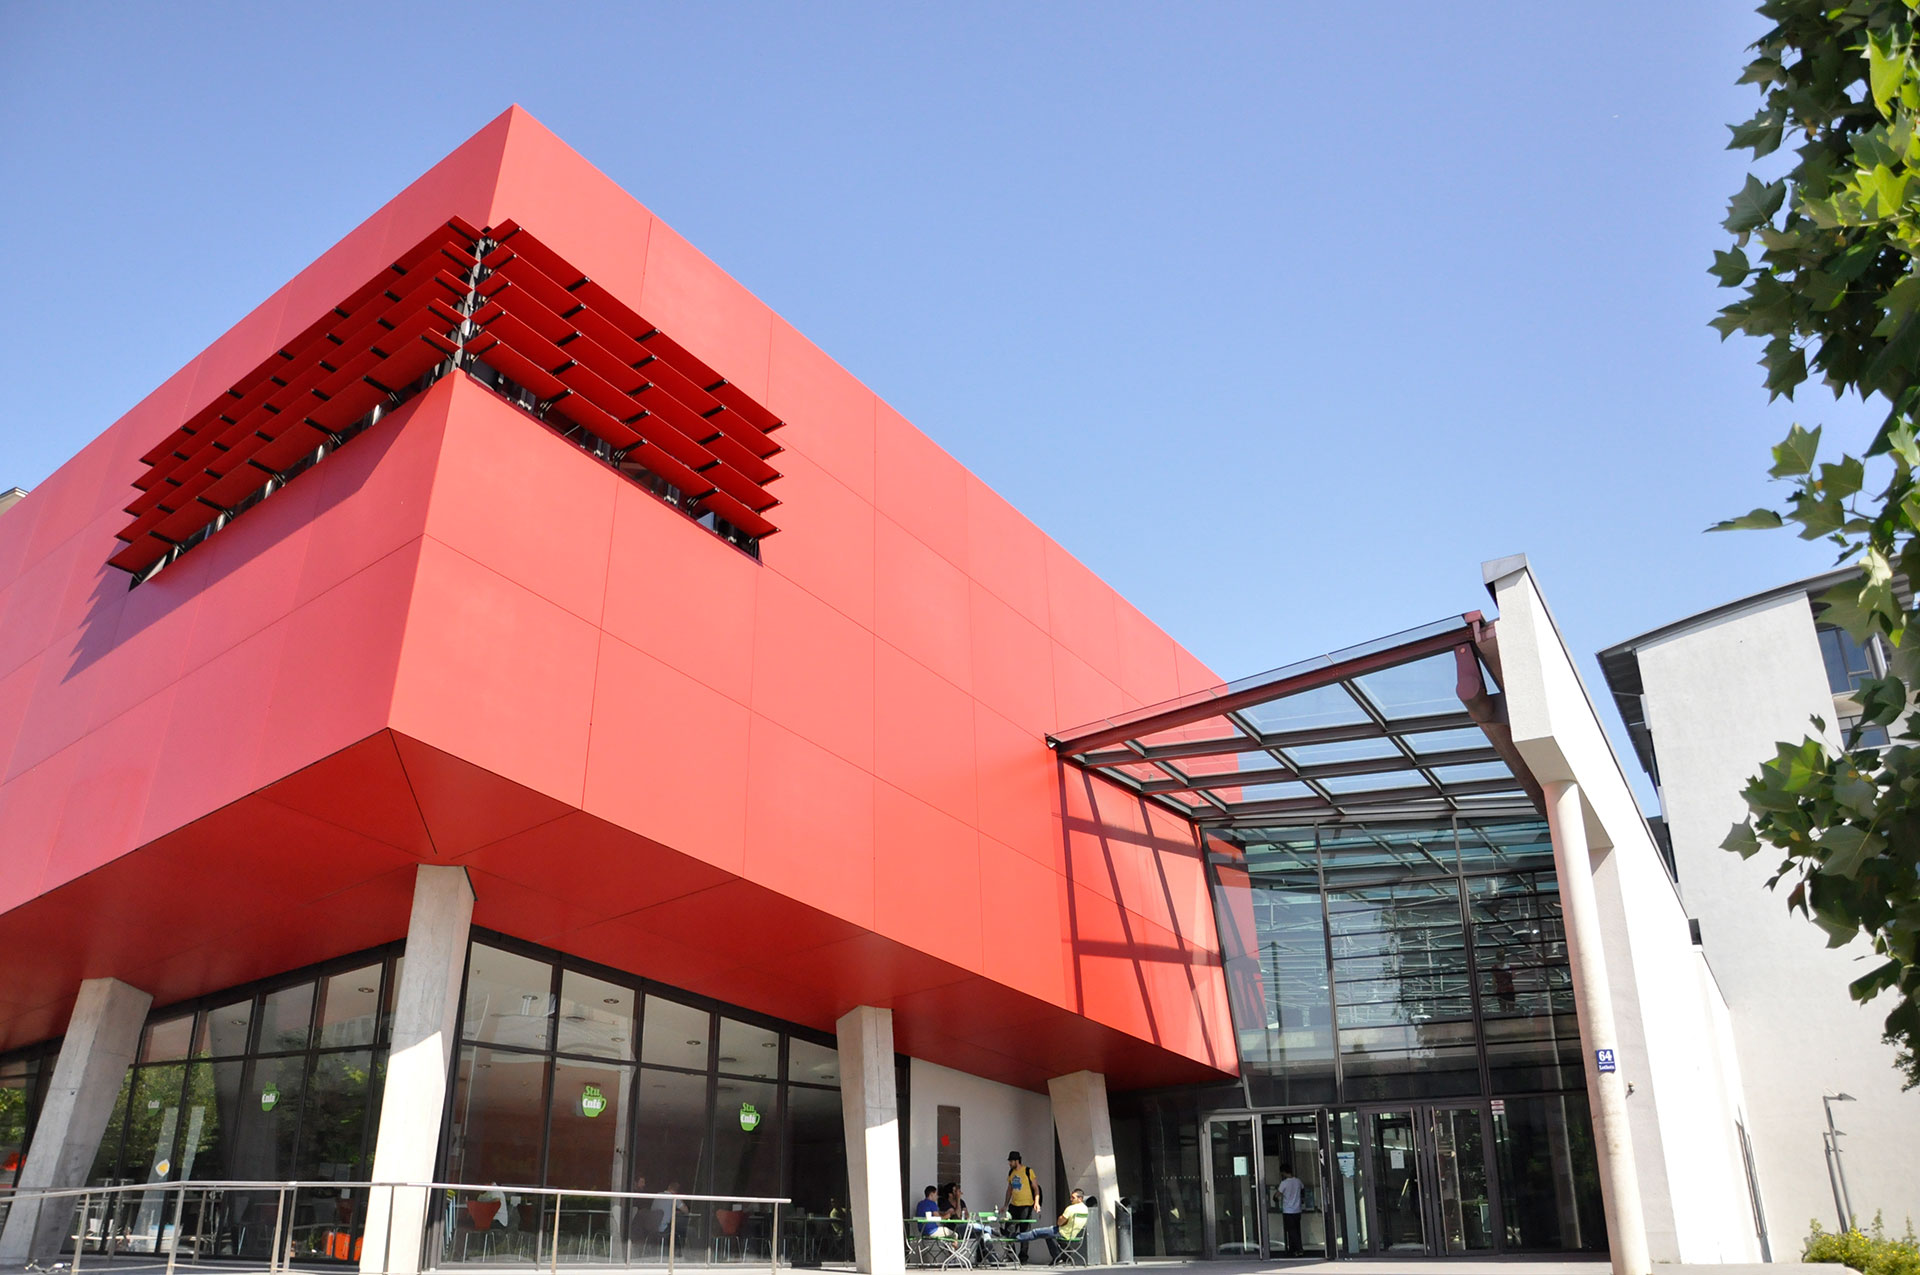
\includegraphics[width=\textwidth]{assets/dm_roter_wuerfel_ben_steinig.jpg}
      \caption{Vorher: Ausgangssituation}
    \end{figure}
  \end{column}
  \hfill
  \begin{column}{0.48\textwidth}
    \begin{figure}
      \centering
      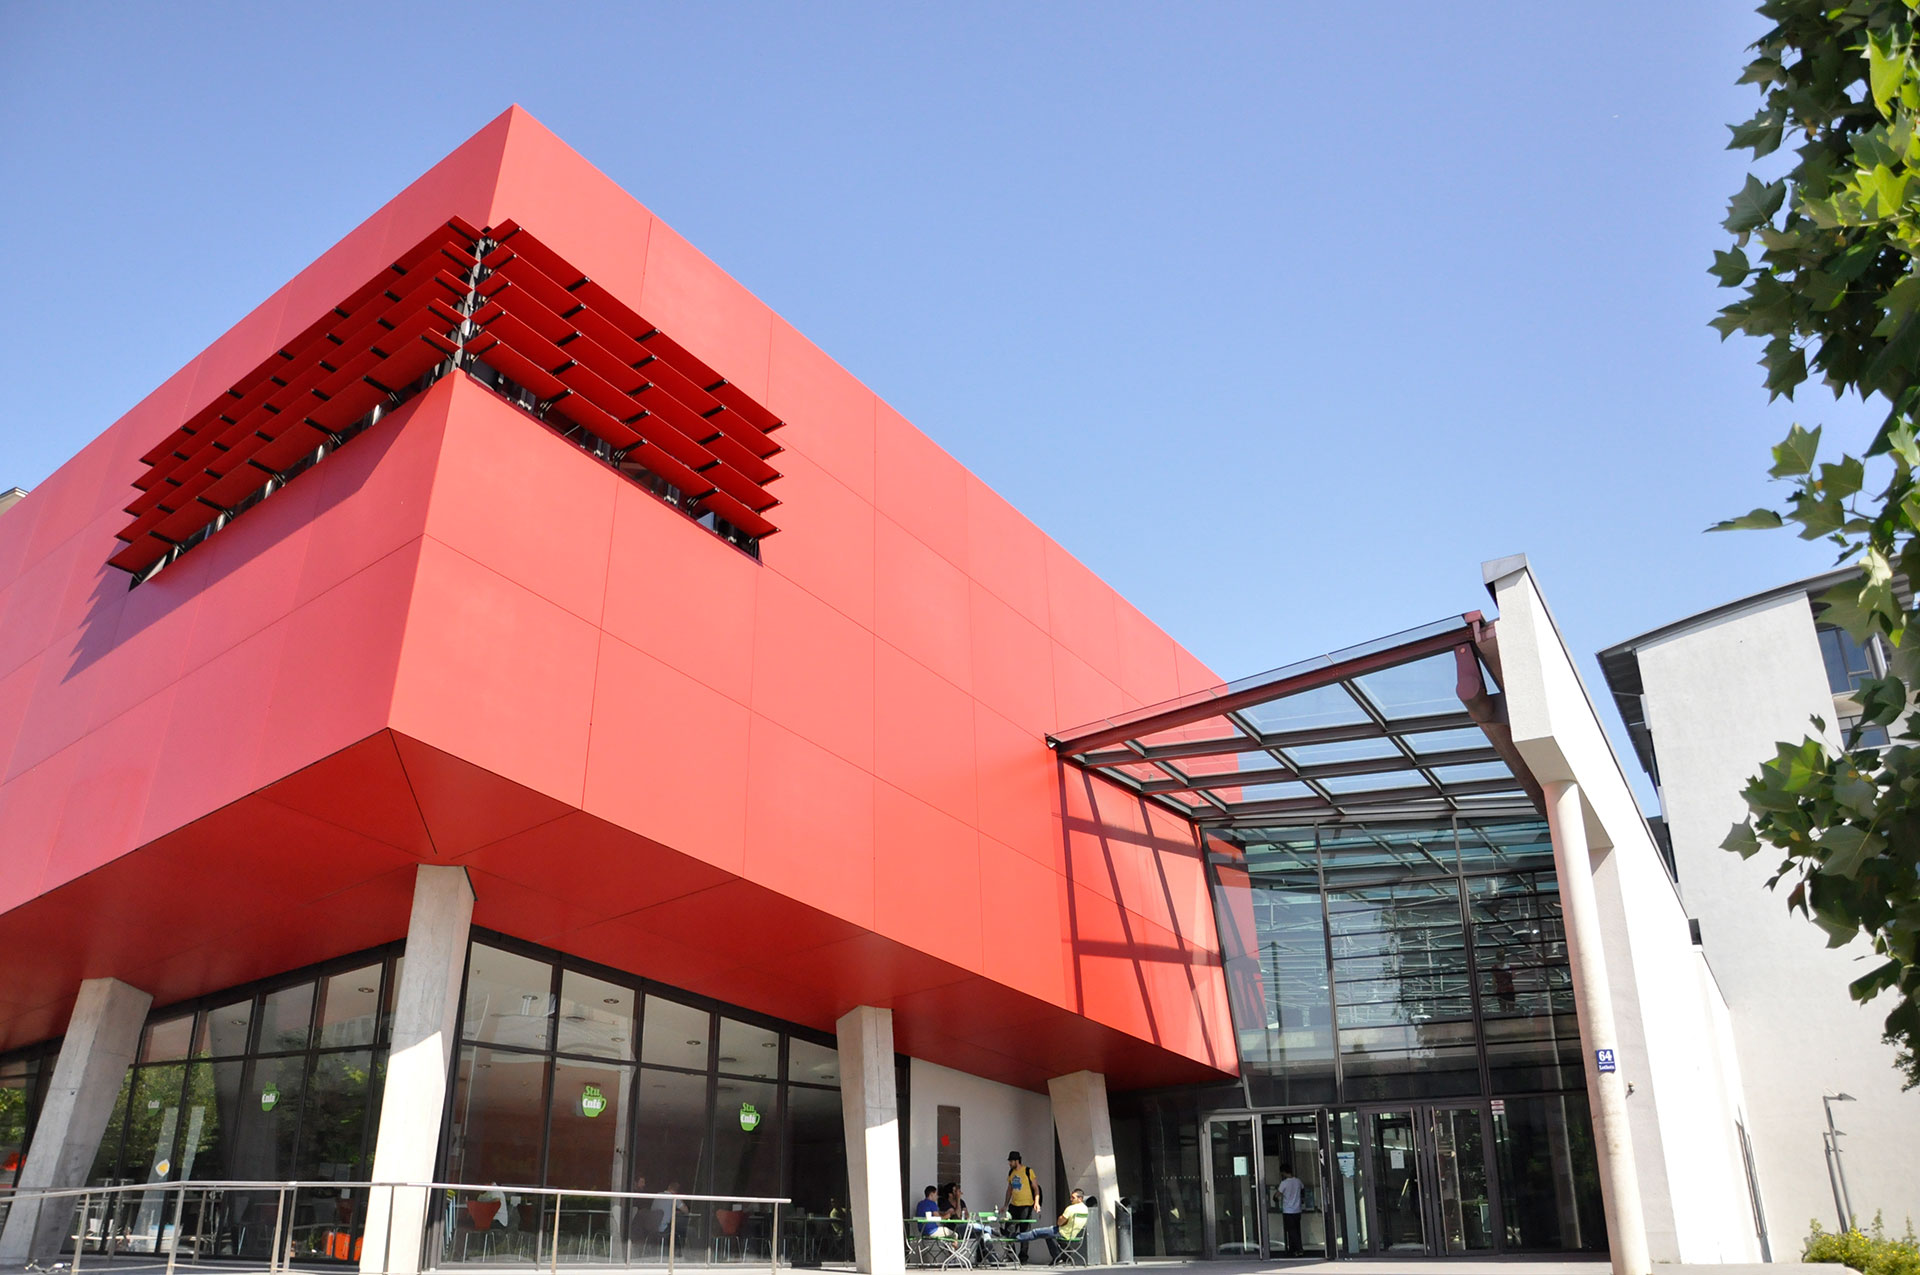
\includegraphics[width=\textwidth]{assets/dm_roter_wuerfel_ben_steinig.jpg}
      \caption{Nachher: Optimierter Zustand}
    \end{figure}
  \end{column}
\end{columns}
\end{frame}

\begin{frame}{Großes Vollbild}
\begin{figure}
  \centering
  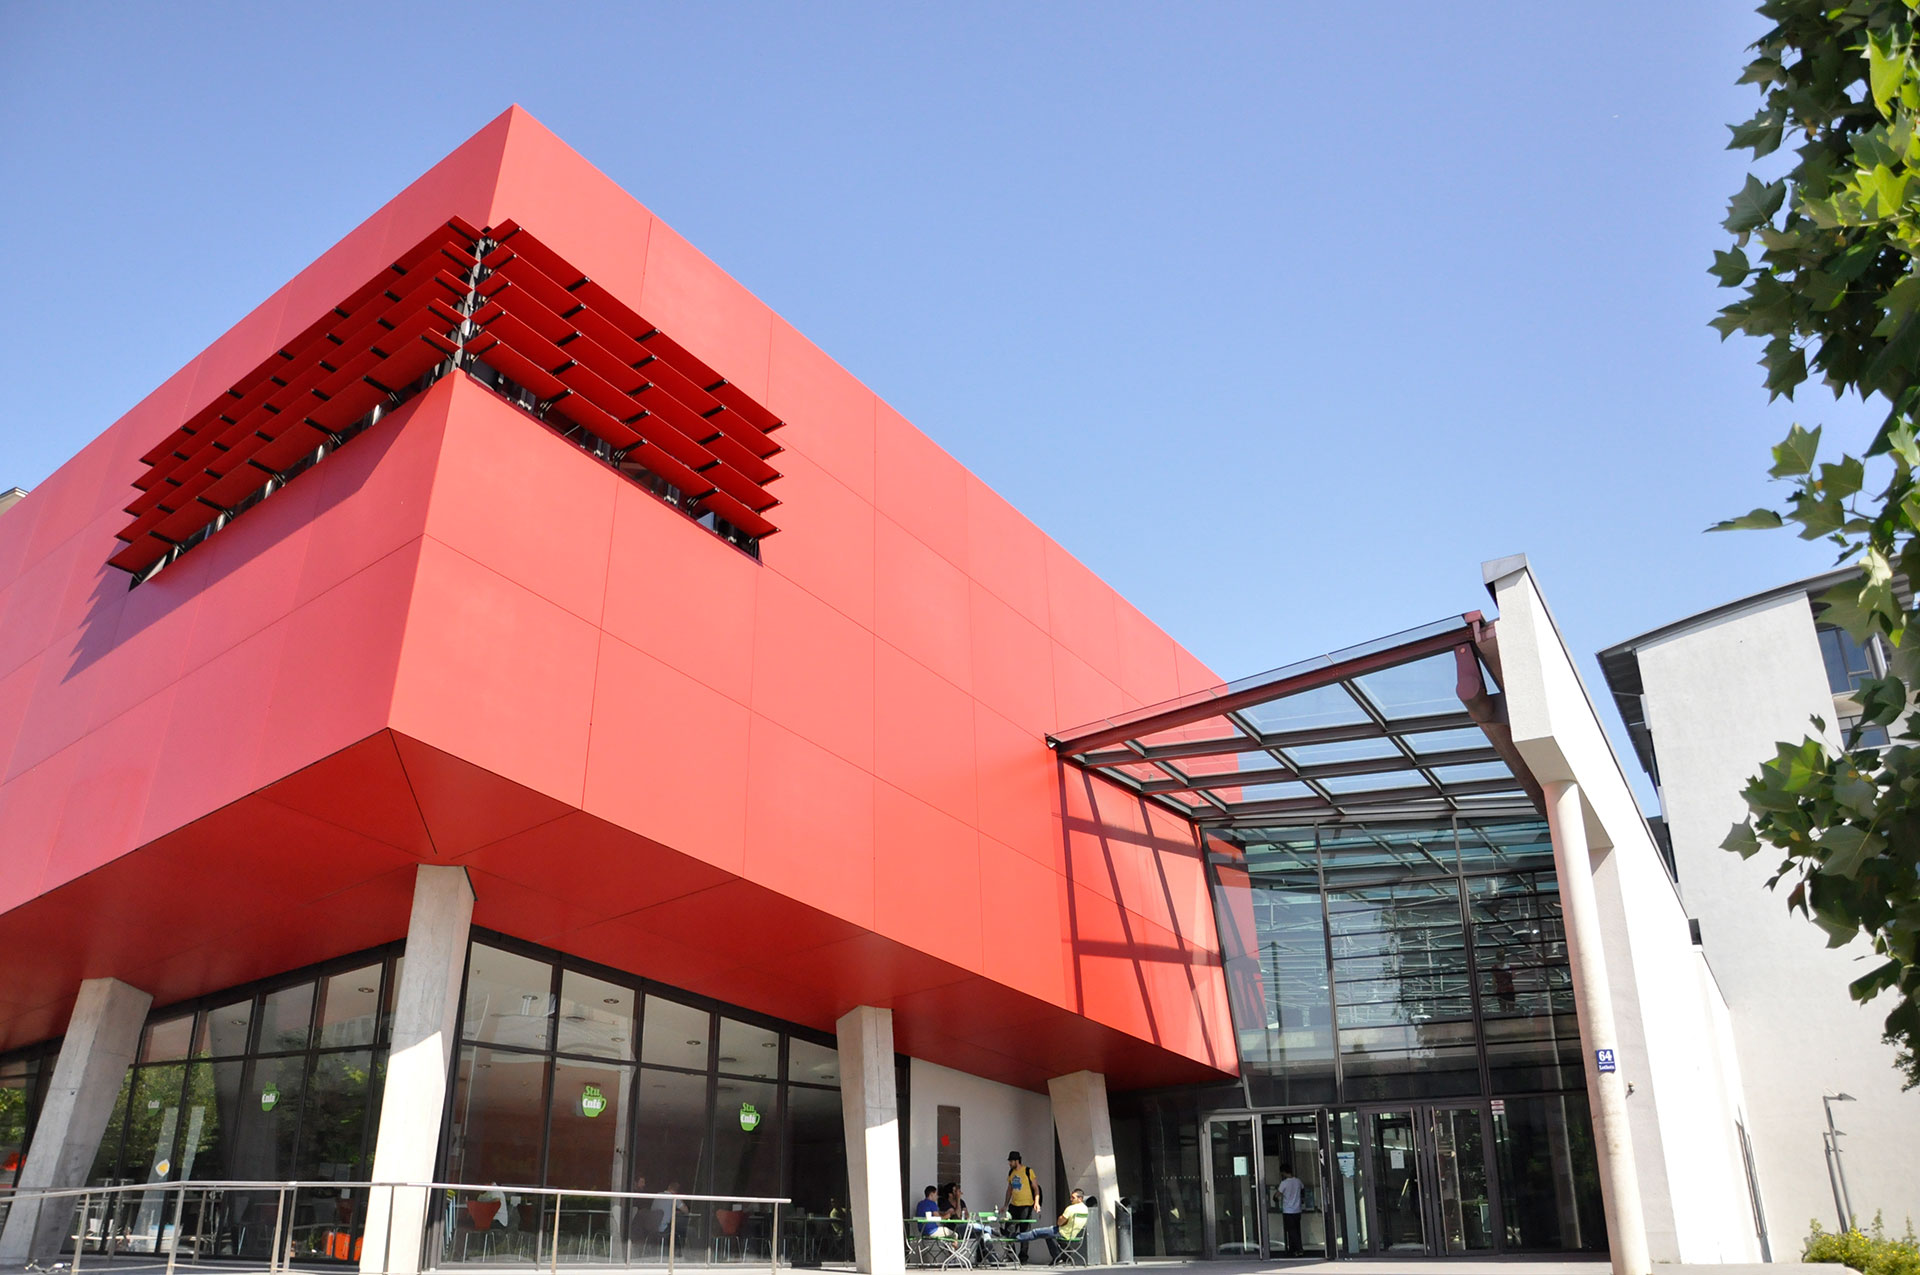
\includegraphics[width=0.9\textwidth,height=0.75\textheight,keepaspectratio]{assets/dm_roter_wuerfel_ben_steinig.jpg}
  \caption{Maximale Bildgröße für starke visuelle Wirkung}
\end{figure}
\end{frame}

\section{Tabellen}
\begin{frame}{Tabelle mit Daten}
\begin{table}
  \centering
  \caption{Übersicht wichtiger Kennzahlen}
  \begin{tabular}{lcc}
    \toprule
    \textbf{Kategorie} & \textbf{2024} & \textbf{2025} \\
    \midrule
    Umsatz (Mio. €) & 45,2 & 52,8 \\
    Wachstum (\%) & 8,5 & 16,8 \\
    Marktanteil (\%) & 12,3 & 14,7 \\
    \bottomrule
  \end{tabular}
\end{table}
\end{frame}

\section{Zitate und Hervorhebungen}
\begin{frame}{Zitat}
\begin{quote}
  \large
  „Ein aussagekräftiges Zitat kann eine Präsentation bereichern und wichtige Botschaften unterstreichen."
\end{quote}
\vspace{0.5cm}
\begin{flushright}
  --- Autor oder Quelle
\end{flushright}
\end{frame}

\begin{frame}{Wichtige Aussage hervorheben}
\begin{center}
  \vspace{1cm}
  {\Huge \textcolor{HMRed}{\textbf{75\%}}}
  
  \vspace{0.5cm}
  {\Large Steigerung der Effizienz}
  
  \vspace{0.5cm}
  durch Optimierung der Prozesse
\end{center}
\end{frame}

\section{Listen und Strukturen}
\begin{frame}{Nummerierte Liste}
\textbf{Schritt-für-Schritt Anleitung:}
\begin{enumerate}
  \item Analyse der Ausgangssituation
  \item Definition der Ziele und Anforderungen
  \item Entwicklung eines Lösungskonzepts
  \item Implementation und Testing
  \item Roll-out und Dokumentation
\end{enumerate}
\end{frame}

\begin{frame}{Verschachtelte Listen}
\begin{itemize}
  \item \textbf{Hauptpunkt 1}
  \begin{itemize}
    \item Unterpunkt A
    \item Unterpunkt B
  \end{itemize}
  \item \textbf{Hauptpunkt 2}
  \begin{itemize}
    \item Unterpunkt C mit weiteren Details
    \item Unterpunkt D
  \end{itemize}
  \item \textbf{Hauptpunkt 3}
\end{itemize}
\end{frame}

\section{Mehrspaltige Inhalte}
\begin{frame}{Drei Spalten}
\begin{columns}[T]
  \begin{column}{0.3\textwidth}
    \centering
    \textbf{\textcolor{HMRed}{Phase 1}}
    
    \vspace{0.3cm}
    Planung und Konzeption
  \end{column}
  \begin{column}{0.3\textwidth}
    \centering
    \textbf{\textcolor{HMRed}{Phase 2}}
    
    \vspace{0.3cm}
    Umsetzung und Testing
  \end{column}
  \begin{column}{0.3\textwidth}
    \centering
    \textbf{\textcolor{HMRed}{Phase 3}}
    
    \vspace{0.3cm}
    Evaluation und Optimierung
  \end{column}
\end{columns}
\end{frame}

\begin{frame}{Gemischtes Layout: Text, Liste und Bild}
\begin{columns}[T]
  \begin{column}{0.55\textwidth}
    \textbf{Projektübersicht}
    
    \vspace{0.3cm}
    Ein komplexes Projekt erfordert strukturierte Planung und klare Kommunikation.
    
    \vspace{0.3cm}
    \textbf{Vorteile:}
    \begin{itemize}
      \item Erhöhte Transparenz
      \item Bessere Nachvollziehbarkeit
      \item Klare Verantwortlichkeiten
    \end{itemize}
  \end{column}
  \begin{column}{0.4\textwidth}
    \begin{figure}
      \centering
      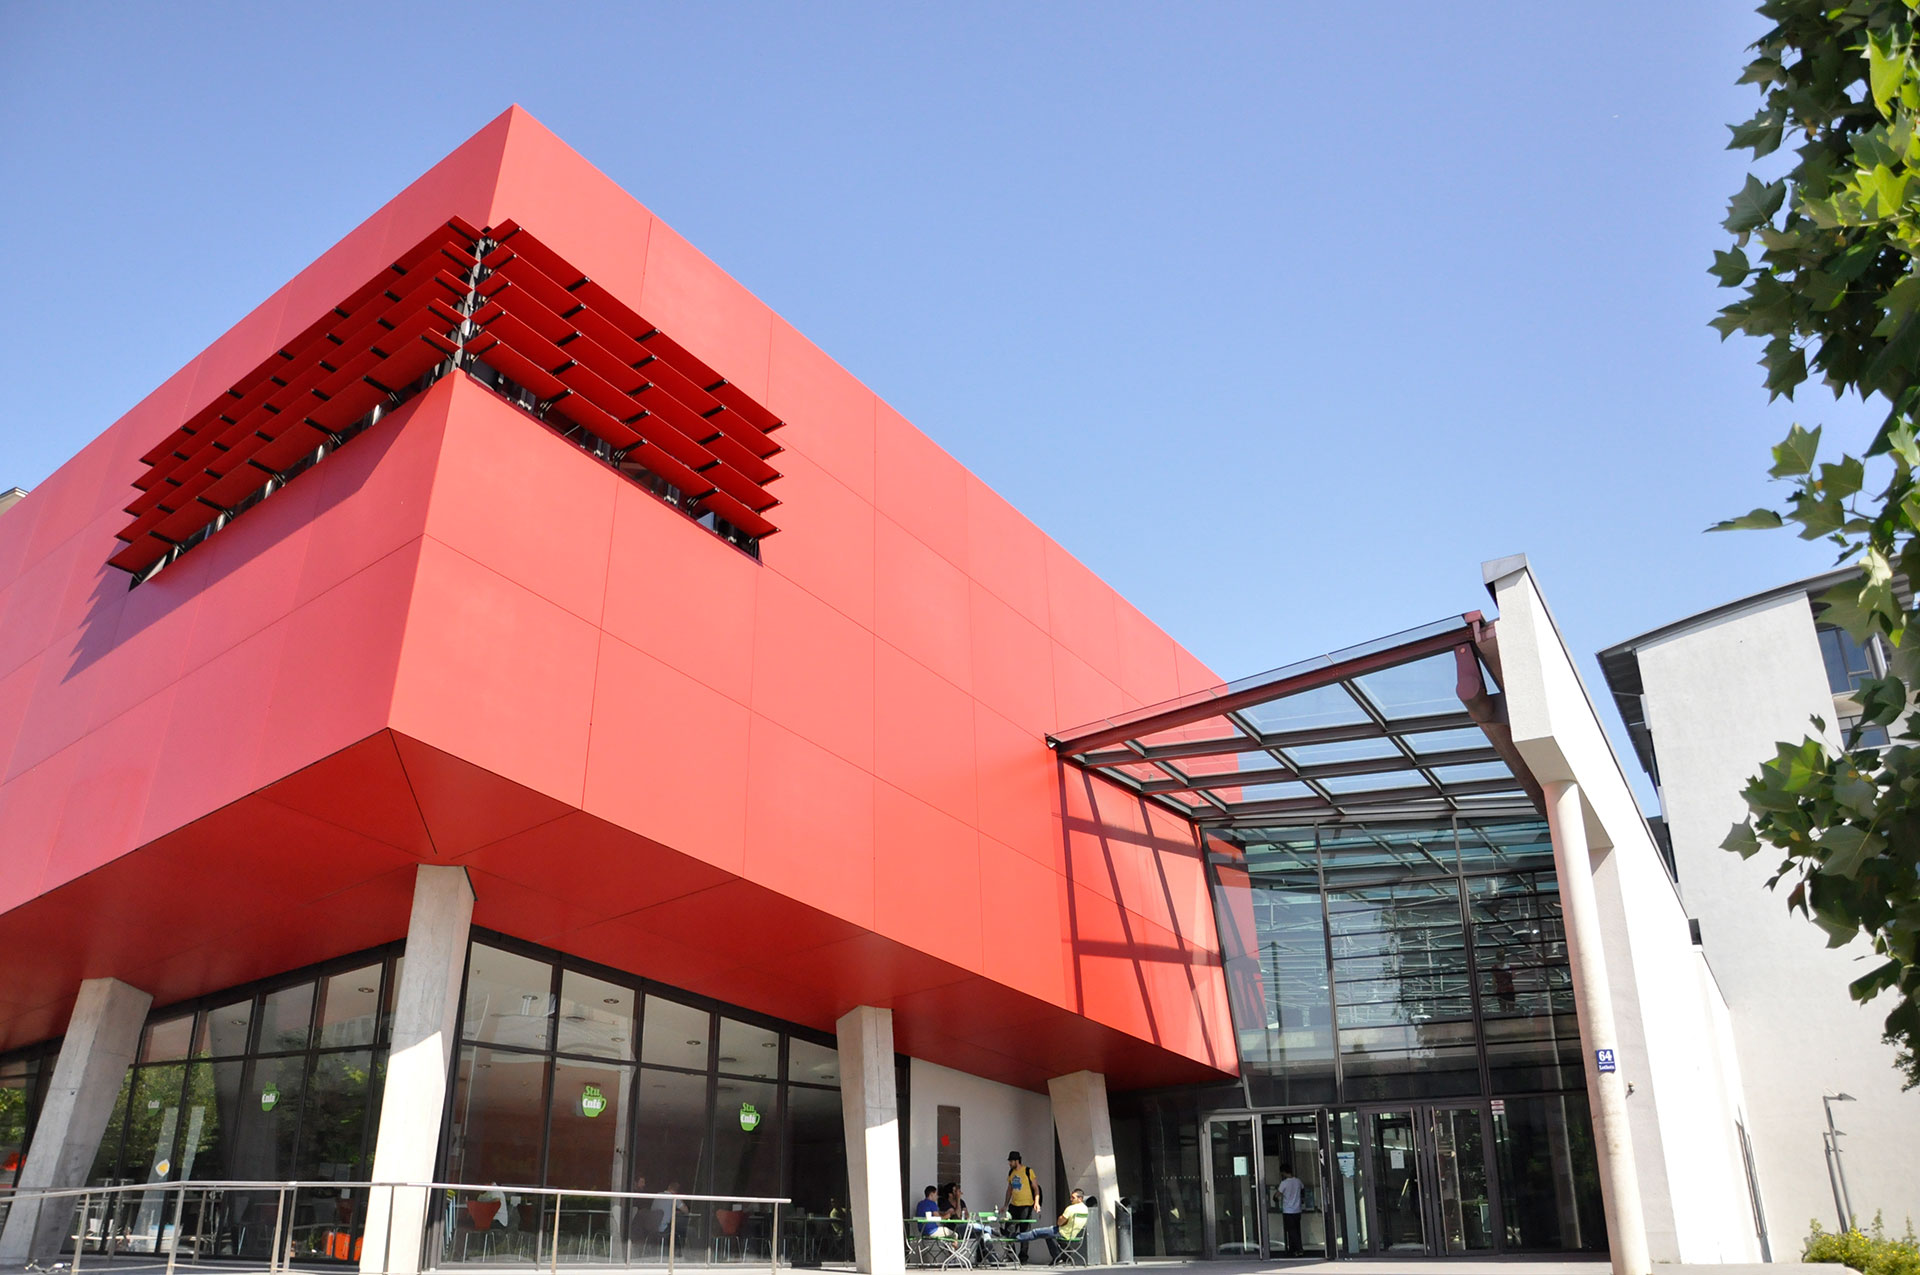
\includegraphics[width=\textwidth]{assets/dm_roter_wuerfel_ben_steinig.jpg}
      \caption{Symbolbild Projekt}
    \end{figure}
  \end{column}
\end{columns}
\end{frame}

\section{Blöcke und Boxen}
\begin{frame}{Verschiedene Blocktypen}
\begin{block}{Standardblock}
  Neutrale Information oder Definition
\end{block}

\begin{exampleblock}{Beispiel}
  Praktisches Anwendungsbeispiel
\end{exampleblock}

\begin{alertblock}{Wichtiger Hinweis}
  Warnung oder besonders wichtige Information
\end{alertblock}
\end{frame}

\begin{frame}{Block mit Liste}
\begin{block}{Erfolgsfaktoren}
  \begin{itemize}
    \item Klare Zielsetzung
    \item Engagiertes Team
    \item Regelmäßiges Monitoring
    \item Offene Kommunikation
  \end{itemize}
\end{block}
\end{frame}

\section{Mathematik und Formeln}
\begin{frame}{Formeln und Berechnungen}
Eine einfache Gleichung:
\[
E = mc^2
\]

\vspace{0.5cm}
Komplexere Berechnungen:
\[
f(x) = \int_{-\infty}^{\infty} e^{-x^2} \, dx = \sqrt{\pi}
\]

\vspace{0.3cm}
Inline-Mathematik: Die Lösung ist $x = \frac{-b \pm \sqrt{b^2-4ac}}{2a}$
\end{frame}

\section{Quellenangaben}
\begin{frame}{Quellen und Referenzen}
\small
\textbf{Literatur:}
\begin{itemize}
  \item Müller, A. (2024): \textit{Effektive Präsentationen}. München: Fachverlag.
  \item Schmidt, B. \& Weber, C. (2023): „Visuelle Kommunikation in der Wissenschaft". \textit{Journal of Communication}, 15(3), S. 234--256.
  \item Online-Quelle: \url{https://www.beispiel.de/artikel}
\end{itemize}
\end{frame}

\begin{frame}{Quellen und Referenzen}
\small
\textbf{Bildquellen:}
\begin{itemize}
  \item Abbildung 1: Eigene Darstellung
  \item Abbildung 2--4: Creative Commons Lizenz
\end{itemize}
\end{frame}

\section{Zusammenfassung}
\begin{frame}{Zusammenfassung}
\begin{itemize}
  \item Fassen Sie die Kernaussagen zusammen und leiten Sie zu nächsten Schritten über.
  \item Nutzen Sie optional die Akzentfarbe \textcolor{HMRed}{HM-Rot} für Highlights.
  \item Schließen Sie mit einem klaren Call-to-Action oder einer Kontaktinformation.
\end{itemize}
\end{frame}

\begin{frame}[plain]
\begin{center}
  \vspace{2cm}
  {\Huge \textbf{Vielen Dank!}}
  
  \vspace{1cm}
  {\Large Fragen und Diskussion}
  
  \vspace{1.5cm}
  \textbf{Kontakt:}\\
  vorname.nachname@hm.edu
\end{center}
\end{frame}

\end{document}